\documentclass[aspectratio=169,11pt]{beamer}

\usetheme{Madrid}
\usecolortheme{default}
\usefonttheme{professionalfonts}
\setbeamertemplate{navigation symbols}{}
\setbeamertemplate{footline}[frame number]

\usepackage{amsmath, amssymb, booktabs, graphicx}
\graphicspath{{../../assets/figures/}{assets/figures/}}

\title{Search, Matching, Turnover, and Unemployment}
\subtitle{Labor II --- Week 4}
\author{Teaching deck draft}
\date{}

\begin{document}

\begin{frame}
  \titlepage
\end{frame}

\begin{frame}{Central question and course repositioning}
\begin{itemize}
    \item Once workers and firms must search for each other, how are hiring, turnover, and unemployment jointly determined?
    \item Week 4 is the first major market-interaction week in Labor II.
    \item The focus is worker flows, vacancies, job ladders, and unemployment dynamics rather than internal firm organization alone.
\end{itemize}
\end{frame}

\begin{frame}{Week 3 to Week 4 bridge}
\begin{itemize}
    \item Week 3 studied incentives, promotions, retention, and internal labor markets inside the firm.
    \item Week 4 asks how quits, layoffs, recruitment, and mobility aggregate into labor-market flows across firms and states.
    \item Week 5 will add wage posting, bargaining, and wage-setting once outside options are fully in view.
\end{itemize}
\end{frame}

\begin{frame}{Why search frictions matter}
\begin{itemize}
    \item Workers do not meet vacancies costlessly.
    \item Jobs end, new jobs open, and many moves happen directly from job to job.
    \item Unemployment is a flow equilibrium outcome, not a static leftover stock.
\end{itemize}
\end{frame}

\begin{frame}{Course map}
\begin{center}
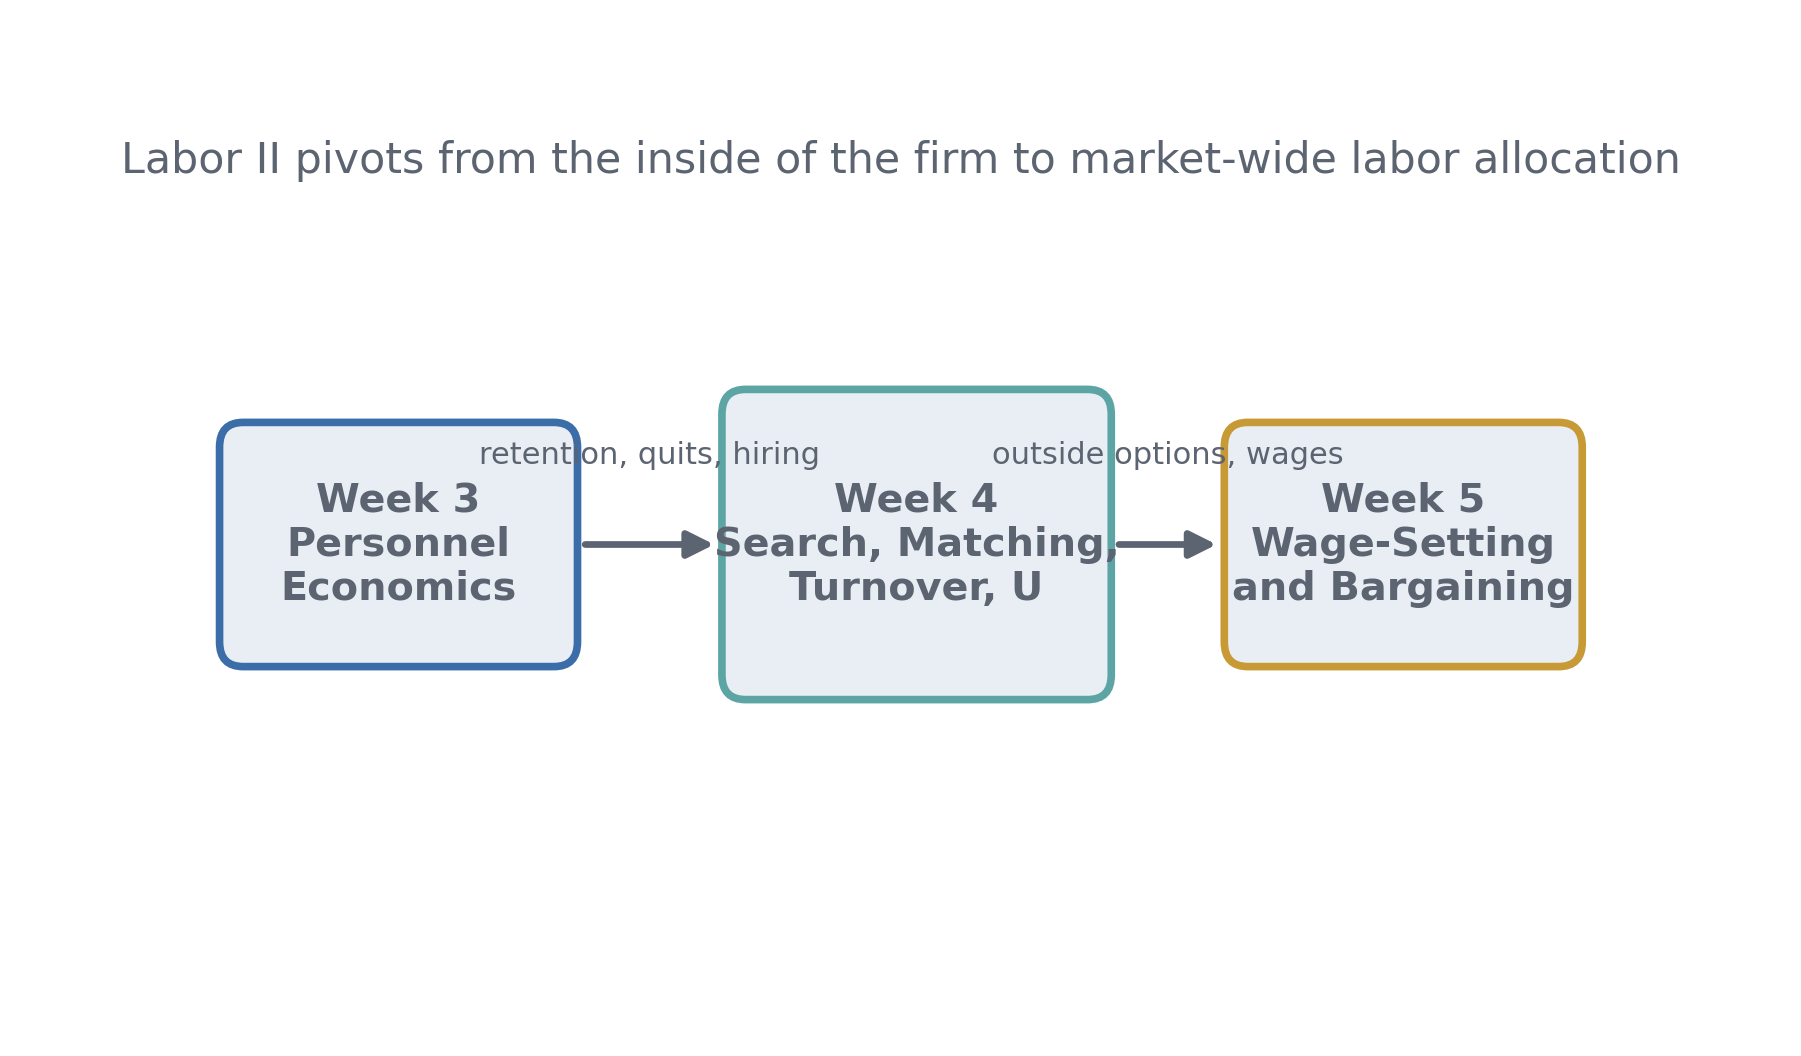
\includegraphics[width=0.9\linewidth]{04-search-course-map.png}
\end{center}
\end{frame}

\begin{frame}{Matching function and worker-side versus vacancy-side hazards}
\[
M_t = \mathcal{M}(U_t, V_t),
\qquad
f_t = \frac{M_t}{U_t},
\qquad
q_t = \frac{M_t}{V_t}
\]

\begin{itemize}
    \item The same meeting technology implies different hazards for workers and firms.
    \item $f_t$ is a job-finding rate; $q_t$ is a vacancy-filling rate.
    \item Matching is a reduced-form meeting object, not yet a full wage or sorting theory.
\end{itemize}
\end{frame}

\begin{frame}{Worker flows and hazards}
\begin{center}
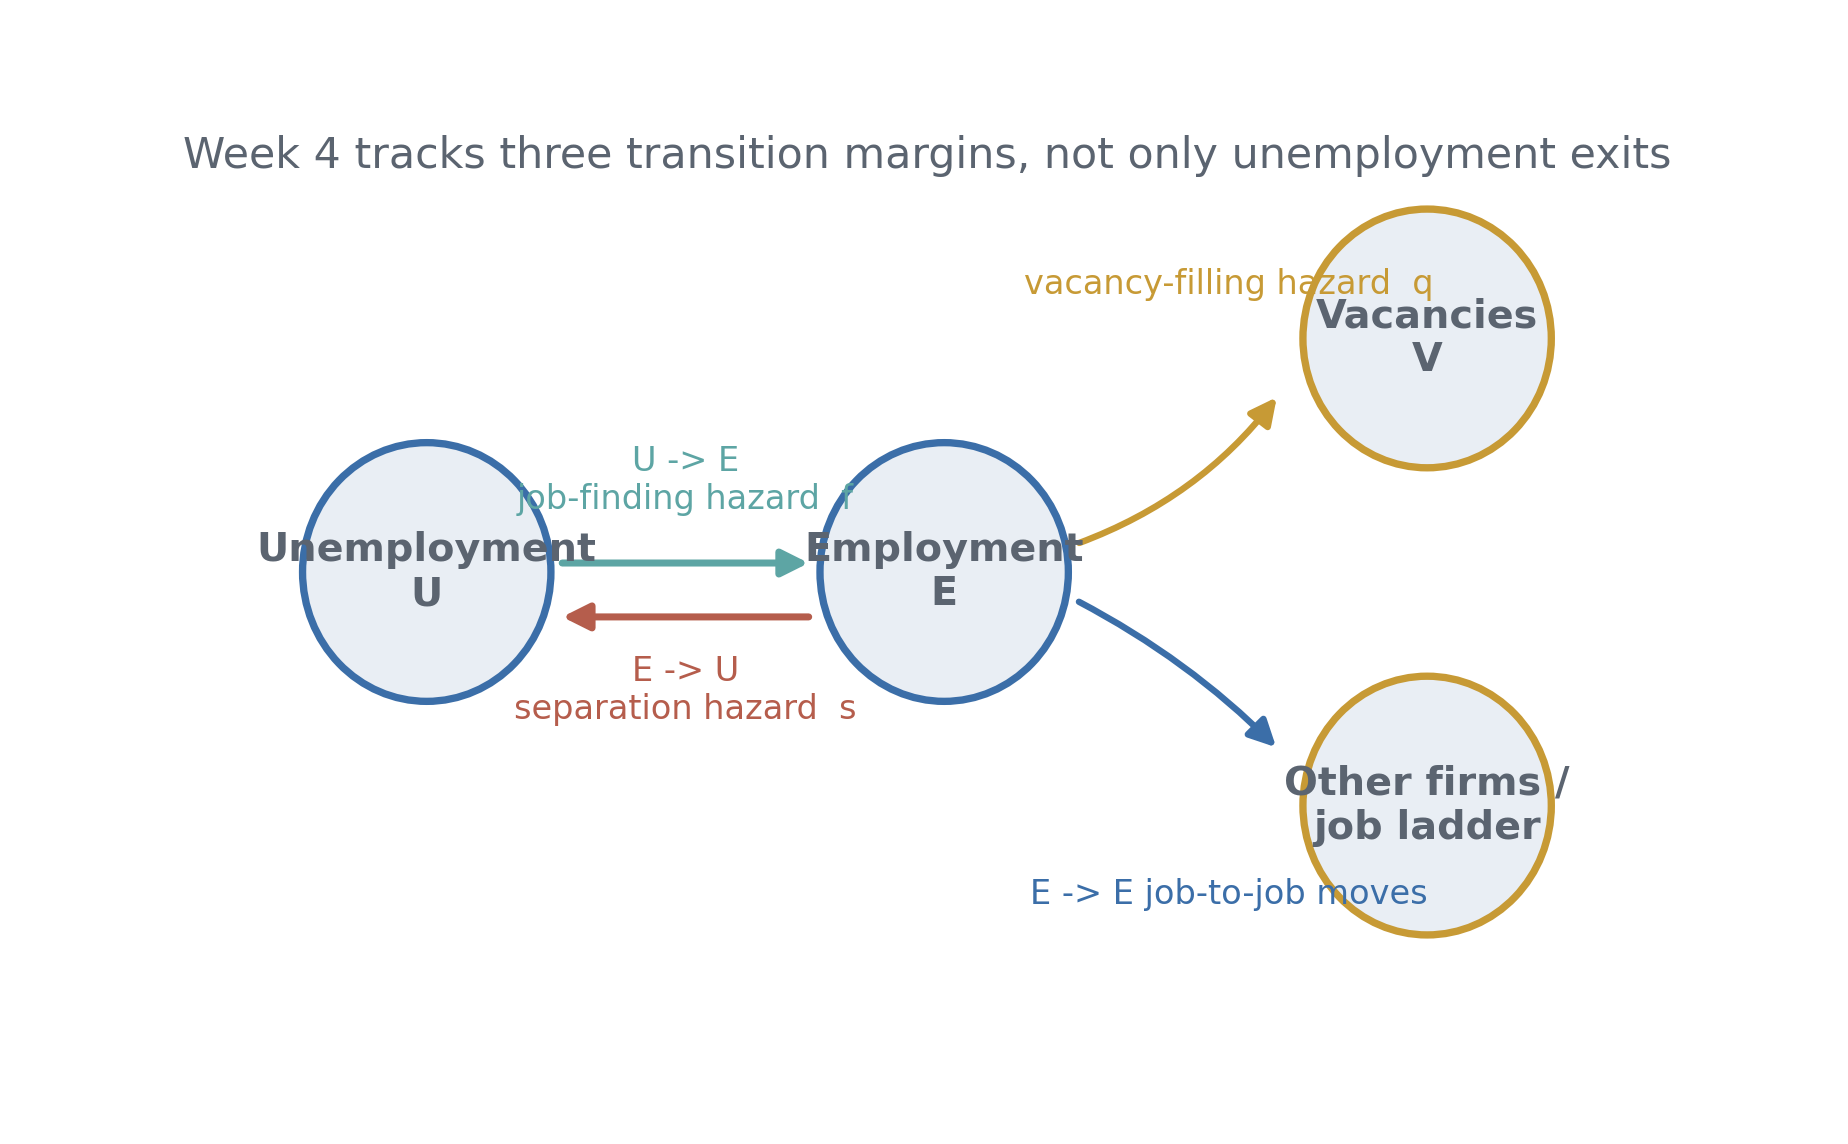
\includegraphics[height=0.7\textheight]{04-worker-flows-and-hazards.png}
\end{center}
\end{frame}

\begin{frame}{Flow unemployment and steady-state accounting}
\[
u_{t+1} - u_t = s_t (1-u_t) - f_t u_t
\]

\[
u^\ast = \frac{s}{s+f}
\]

\begin{itemize}
    \item Unemployment depends jointly on inflows from employment and outflows to jobs.
    \item A high-unemployment market can reflect high separations, low job finding, or both.
    \item A theory of unemployment without separations is incomplete.
\end{itemize}
\end{frame}

\begin{frame}{Beveridge logic and matching efficiency}
\begin{center}
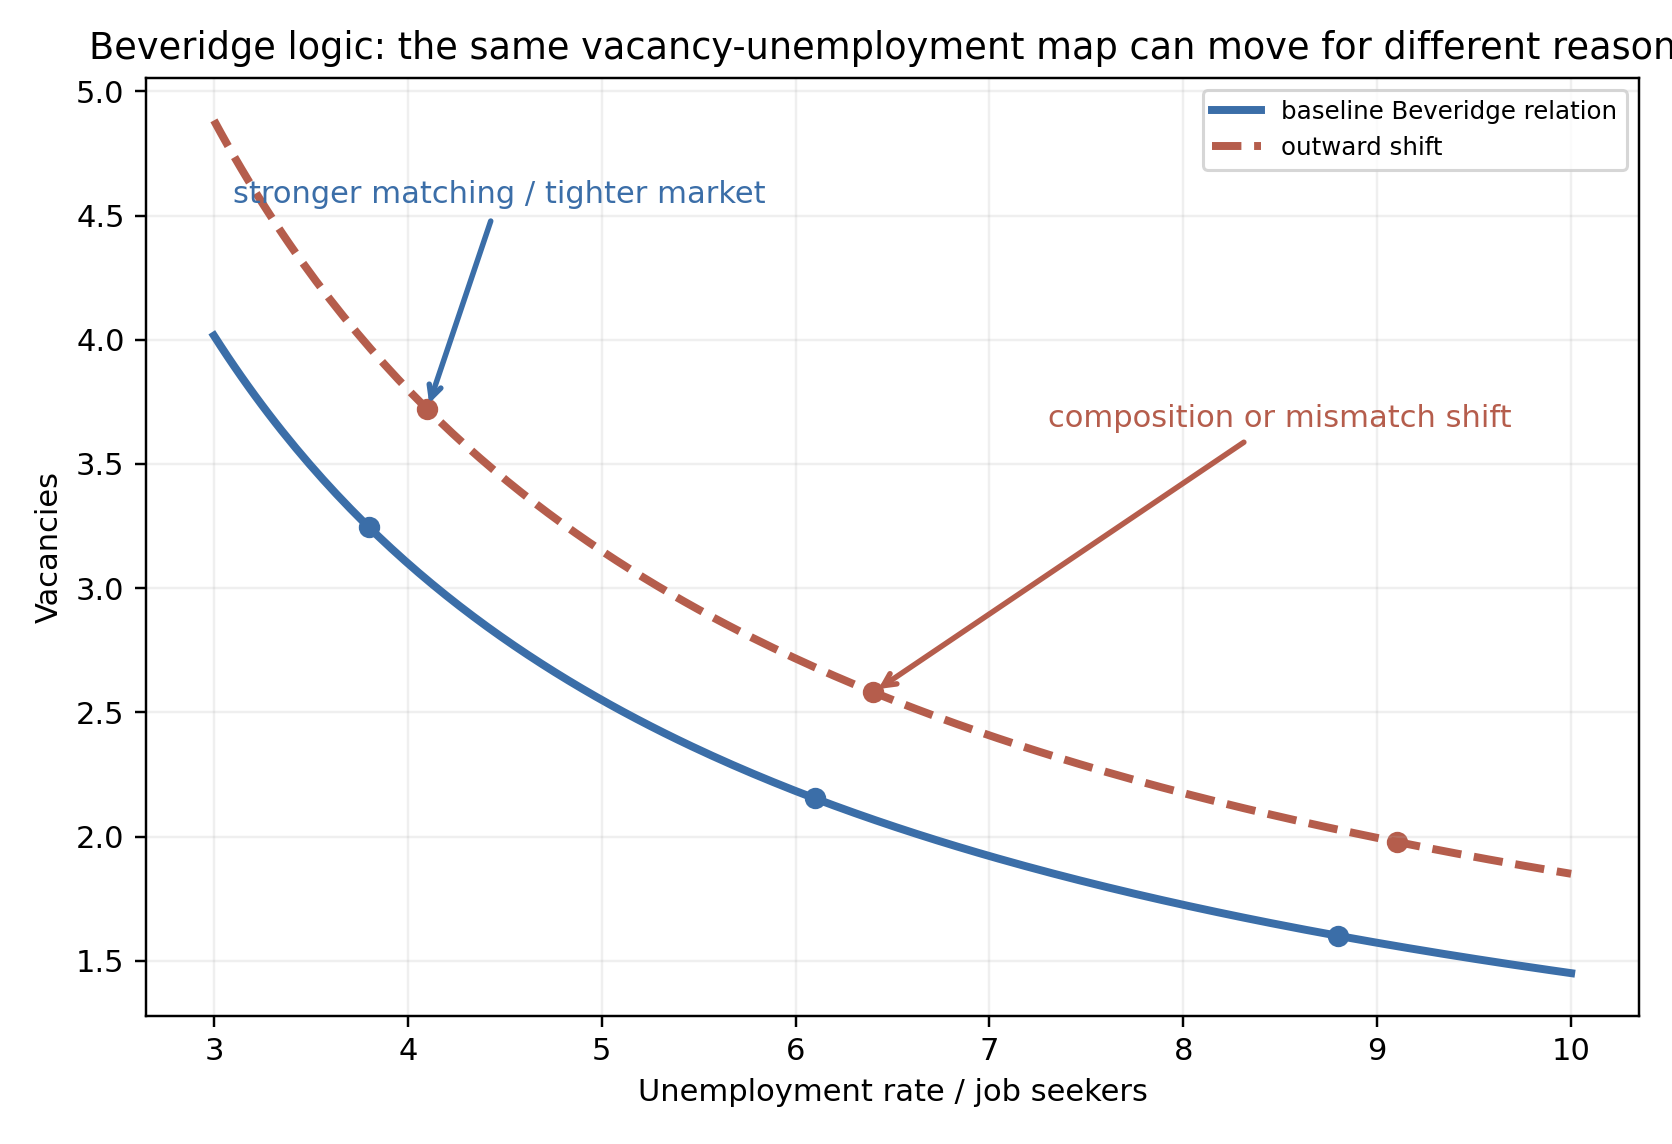
\includegraphics[height=0.68\textheight]{04-beveridge-matching-efficiency.png}
\end{center}
\end{frame}

\begin{frame}{Separations, turnover, layoffs, job destruction, and churning}
\begin{itemize}
    \item A separation ends a worker-firm spell; a layoff is one type of separation.
    \item Job destruction is a job-flow object, not a synonym for worker turnover.
    \item Churning is worker reallocation beyond what net employment change requires.
    \item Stable headcount can hide intense replacement hiring and restructuring.
\end{itemize}
\end{frame}

\begin{frame}{Separations, churning, and job ladders}
\begin{center}
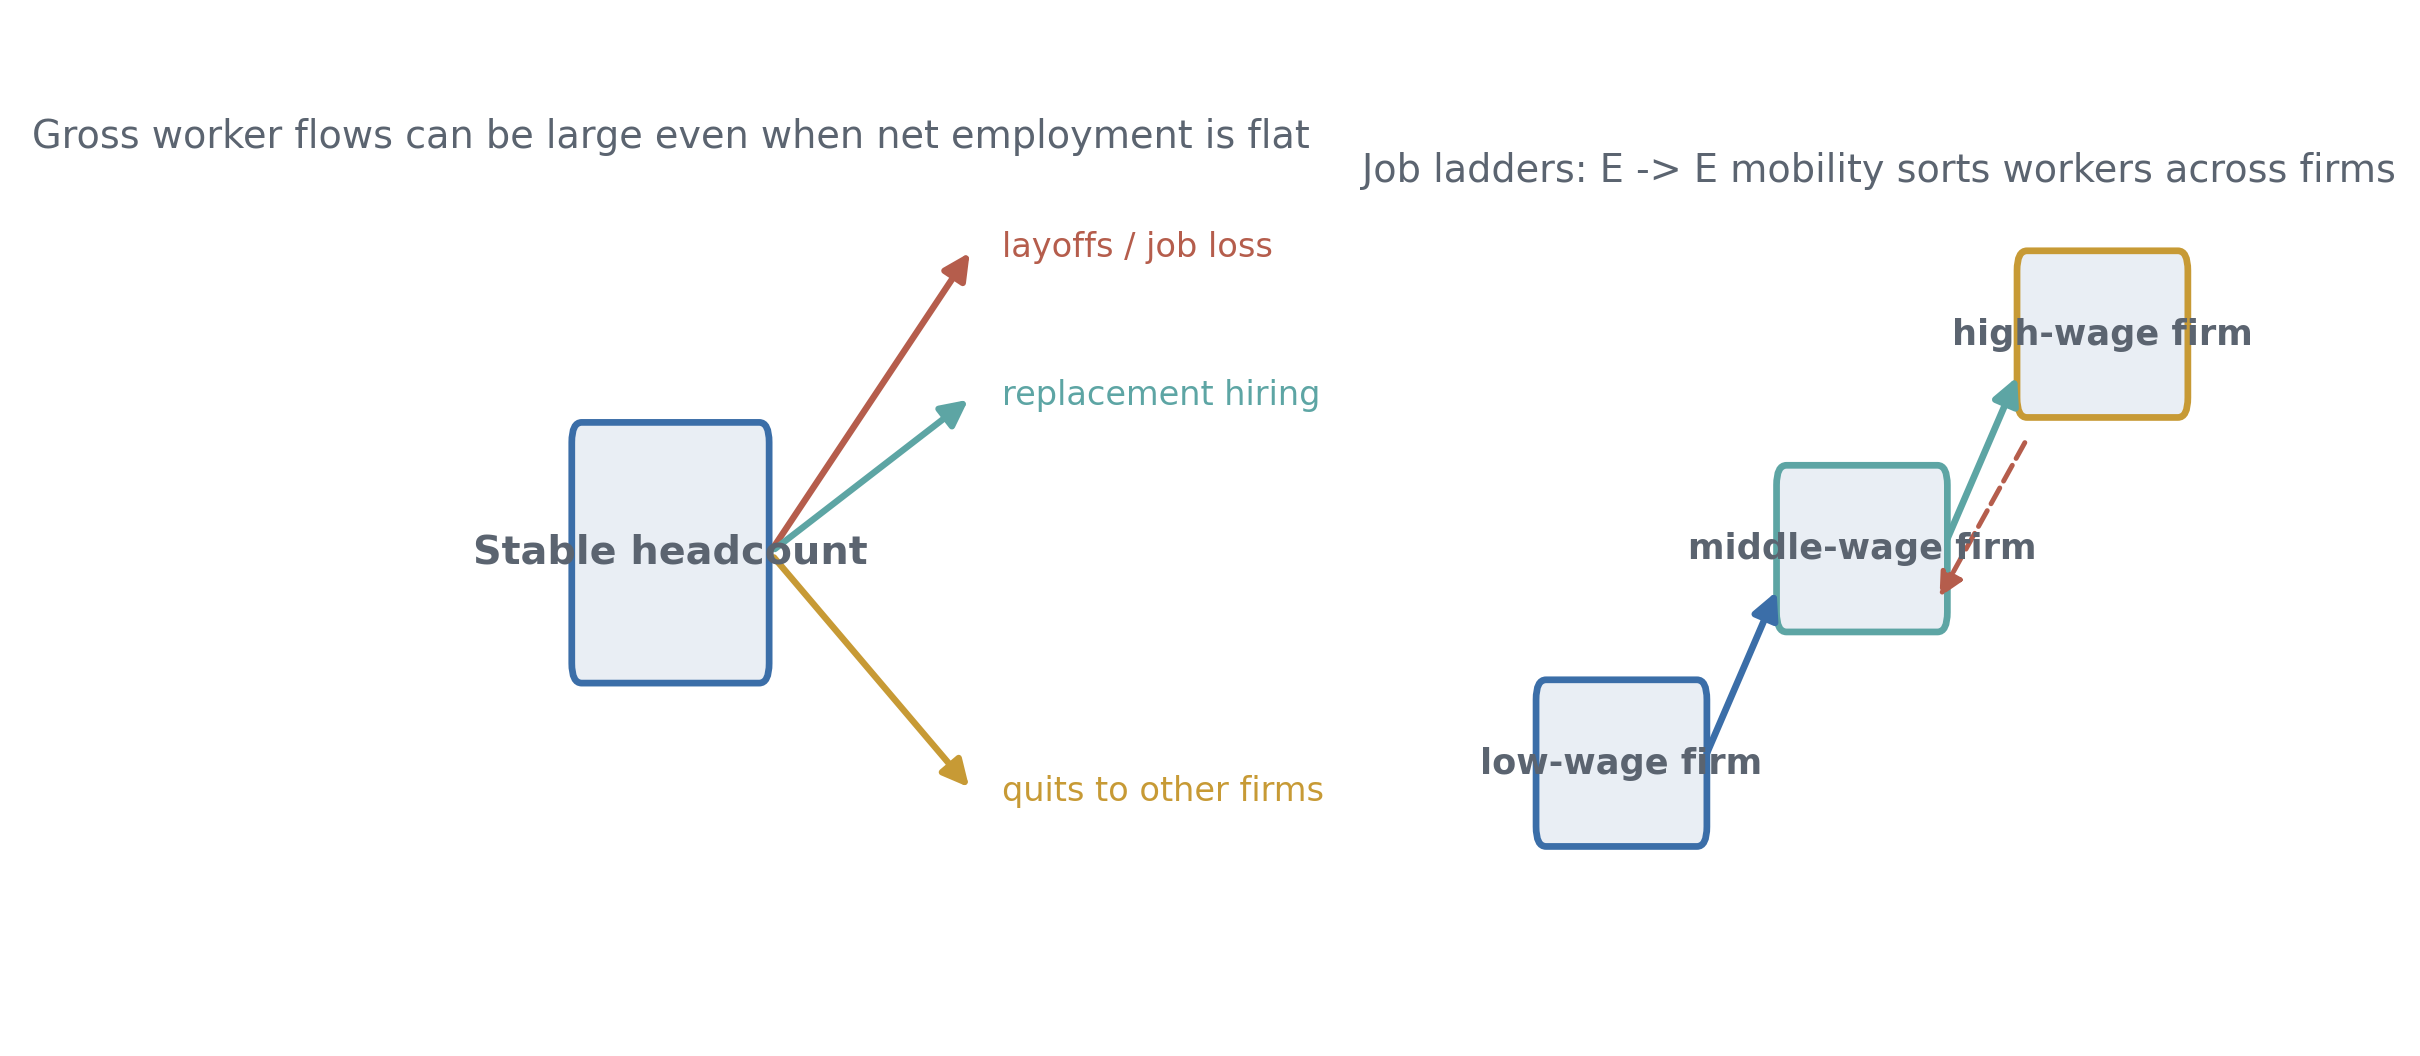
\includegraphics[height=0.68\textheight]{04-separation-churning-jobladder.png}
\end{center}
\end{frame}

\begin{frame}{Job-to-job transitions, on-the-job search, and job ladders}
\[
\lambda^{EE}_{it} = \lambda\big(w_{it}, x_i, \phi_t, \text{firm quality}_j\big)
\]

\begin{itemize}
    \item Many labor-market transitions never pass through unemployment.
    \item Employed search drives poaching, retention pressure, wage growth, and sorting.
    \item Job ladders flatten in weak markets even before all adjustment shows up in unemployment.
\end{itemize}
\end{frame}

\begin{frame}{Unemployment duration, search intensity, and unemployment effects}
\[
y_i^{\text{reemp}} = \alpha + \beta D_i + \gamma X_i + \varepsilon_i
\]

\begin{itemize}
    \item Observed duration dependence is not automatically a causal unemployment effect.
    \item Search intensity, beliefs, employer screening, and dynamic selection can all matter.
    \item The post-unemployment object includes job quality and scarring, not just exit hazards.
\end{itemize}
\end{frame}

\begin{frame}{Duration dependence and scarring}
\begin{center}
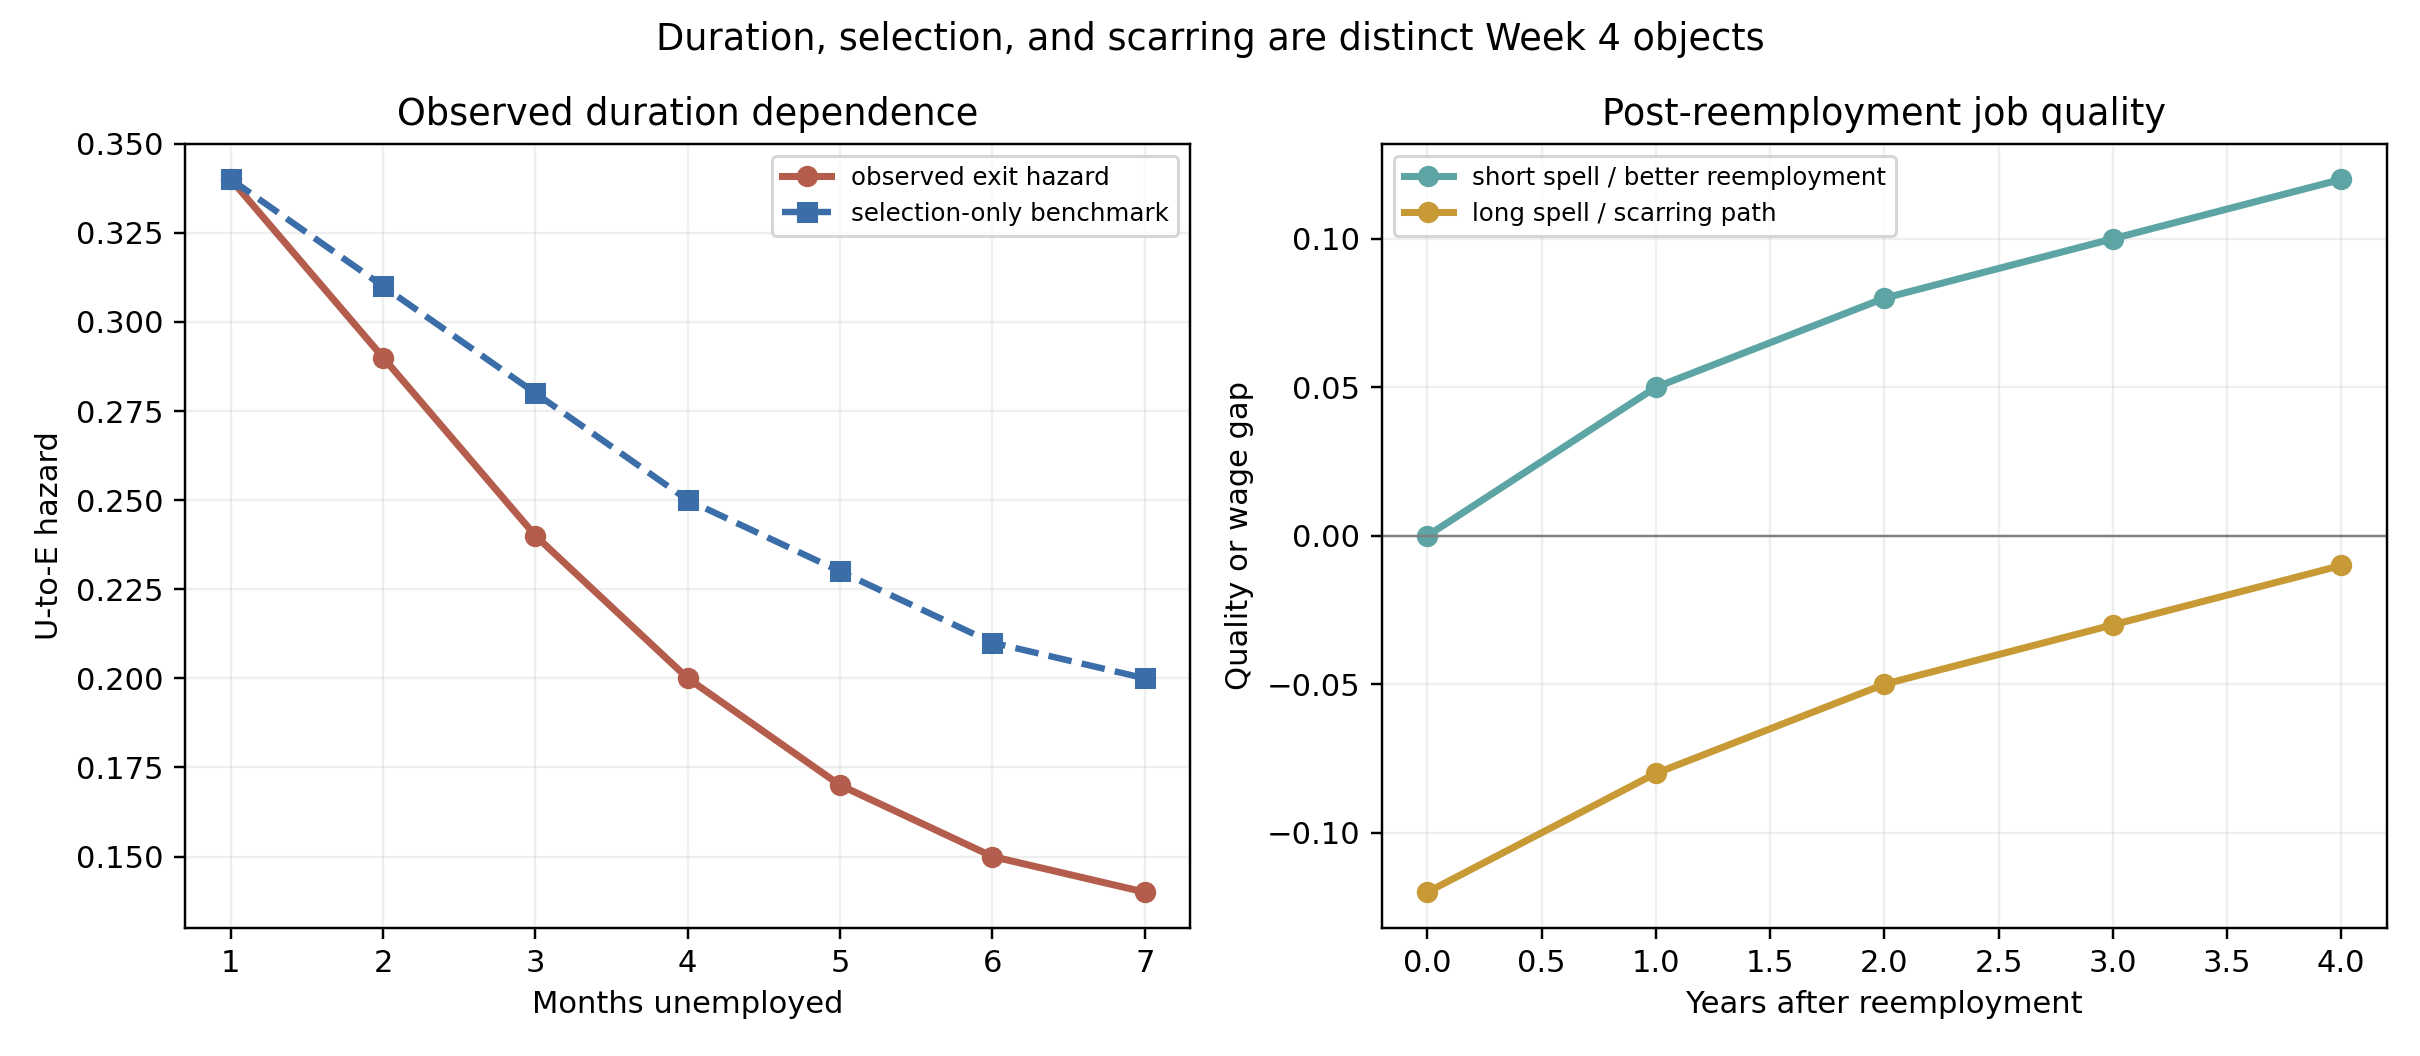
\includegraphics[height=0.68\textheight]{04-unemployment-duration-and-scarring.png}
\end{center}
\end{frame}

\begin{frame}{Empirical designs and what they identify}
\small
\begin{tabular}{p{0.22\linewidth} p{0.23\linewidth} p{0.18\linewidth} p{0.25\linewidth}}
\toprule
Design & Variation & Margin & Hardest unobserved object \\
\midrule
CPS flows & Worker-month transitions & U-E, E-U & Match quality, recruiting intensity \\
Vacancy evidence & Time or place vacancies & Vacancy filling, Beveridge shifts & Searcher composition, mismatch \\
Linked worker-firm data & Worker moves across firms & E-E, churning, ladders & Opportunity set, reasons for moves \\
Search-platform data & Applications over spell & Search intensity, targeting & Representativeness \\
Field experiments or policy shocks & Randomized histories, UI rules & Duration, callbacks, job quality & General-equilibrium spillovers \\
\bottomrule
\end{tabular}
\end{frame}

\begin{frame}{Frontier extension}
\begin{itemize}
    \item Beliefs and expectations: perceived hazards shape search effort.
    \item Digital search traces: applications reveal targeting and intensity, but coverage is incomplete.
    \item Selective hiring and mismatch: Beveridge shifts can reflect composition, not just efficiency.
    \item Scarring and firm quality loss: recession timing changes later opportunities and job ladders.
\end{itemize}
\end{frame}

\begin{frame}{Bridge to Week 5 wage-setting}
\begin{itemize}
    \item Once vacancies take time to fill and workers have outside options, the wage is no longer an anonymous competitive parameter.
    \item Search frictions create the environment for wage posting, bargaining, retention pressure, and rent sharing.
    \item Week 5 asks how wages are set once this Week 4 mobility structure is in place.
\end{itemize}
\end{frame}

\begin{frame}{Takeaways}
\begin{itemize}
    \item Search theory is about worker flows, vacancies, separations, mobility, and unemployment jointly.
    \item The key distinctions are U-E versus E-U versus E-E, worker flows versus job flows, and matching efficiency versus composition.
    \item Modern evidence combines transition data, vacancy data, linked worker-firm records, digital search traces, and policy or field variation.
    \item Week 5 turns these mobility and outside-option objects into wage-setting theory.
\end{itemize}
\end{frame}

\end{document}
